\documentclass[11pt, a4paper]{article}

% --- Packages ---
\usepackage[utf8]{inputenc} % Encoding
\usepackage{amsmath, amssymb, amsthm} % Advanced math typesetting
\usepackage{physics} % Useful commands for physics (derivatives, vectors, braket)
\usepackage{graphicx} % For including diagrams and images
\usepackage{geometry} % Page margins
\usepackage{siunitx} % For proper formatting of SI units
\usepackage{fancyhdr} % Custom headers and footers
\usepackage{xcolor} % For blocks of color
\usepackage{enumitem} % For enumerated lists with letters
\usepackage{float} % For figure strict positioning
\usepackage{parskip} % Elimina la sangría y añade espacio entre párrafos
\usepackage{hyperref} % URL suppeort
\usepackage{tikz}
\usepackage{pgfplots}

% --- Page Setup ---
\geometry{top=2.5cm, bottom=2.5cm, left=2.5cm, right=2.5cm}
\pagestyle{fancy}
\fancyhf{} % Clear all default header and footer fields
\fancyhead[L]{\textbf{José Carlos López Henestrosa}}
\fancyhead[R]{Fundamentos físicos de la informática - PEC4}
\fancyfoot[C]{\thepage} % Page number at the bottom center


% --- Custom Environments ---
% Creates a neat "Problem X" environment
% --- Custom Environments ---
\newenvironment{problem}[1][Cuestión]{
	\vspace{0.5cm}
	\noindent{\Large\bfseries #1} \par\vspace{0.5cm}
}{
	\vspace{0.5cm}
}

\begin{document}
	% --- Title Block ---
	\begin{center}
		\Large{ \textbf{PEC4} } \\
		\vspace{0.5cm}
		\normalsize{\textbf{Nombre:} José Carlos López Henestrosa} \\
		\vspace{0.5cm}
		\normalsize{Declaro que ostento la autoría total y llena de todas las tareas que se llevan a cabo en el presente documento. Soy la única persona que ha elaborado cada ejercicio. No he compartido los enunciados con nadie y la única ayuda que he recibido ha sido a través del aula de la UOC y su profesorado y he citado de forma explícita los recursos externos que he usado en la preparación de la PEC.} \\
		\vspace{0.5cm}
		\normalsize{Todas las referencias académicas en esta entrega hacen referencia a los libros \textit{Magnetostática e inducción electromagnética} y \textit{Materiales y dispositivos semiconductores} de los recursos de esta asignatura, salvo que se cite otra fuente explícitamente.}
	\end{center}

	\vspace{1cm}
	\hrule
	\vspace{1cm}

	% --- Exercise 1 ---
	\begin{problem}[Cuestión 1]
		En un experimento de laboratorio, una partícula cargada $P$ con carga $q = 4 \; \mu C$ entra en una región del espacio donde hay un campo magnético uniforme $\vec{B} = 2 \vec{j} - 3 \vec{k} \text{ T}$. En el momento de entrar en esta región, la velocidad de la partícula es $\vec{v} = v_0 \vec{i} + 2 v_0 \vec{k}$, con $v_0 > 0$. Se sabe que el módulo de la fuerza magnética que actúa sobre la partícula es $|\vec{F}_m| = 8 \text{ mN}$. Determine el valor de $v_0$.

		{ \color{blue} 
			\textbf{NOTA:} Todas las fórmulas de esta cuestión han sido tomadas del libro \textit{Magnetostática e inducción electromagnética}.
		}

		{ \color{blue} 
			Para deducir el valor de $v_0$, debemos calcular primero el vector de la fuerza magnética ejercida sobre la carga en movimiento. La ley que relaciona estas variables es la Ecuación 38: $\vec{F}_m = q\vec{v} \wedge \vec{B}$.

			Para desarrollar el producto vectorial entre la velocidad y el campo magnético, utilizamos la resolución por determinantes expresada en la Ecuación 5: $\vec{a} \wedge \vec{b} = \begin{vmatrix} \vec{i} & \vec{j} & \vec{k} \\ a_1 & a_2 & a_3 \\ b_1 & b_2 & b_3 \end{vmatrix}$.

			Aplicando esta ecuación a nuestros datos, tenemos:
			\begin{equation*}
				\vec{v} \wedge \vec{B} = 
				\begin{vmatrix}
					\vec{i} & \vec{j} & \vec{k} \\
					v_0 & 0 & 2v_0 \\
					0 & 2 & -3
				\end{vmatrix}
			\end{equation*}

			Resolviendo el determinante, obtenemos el siguiente vector:
			\begin{align*}
				\vec{v} \wedge \vec{B} &= \vec{i} \cdot (0 \cdot (-3) - 2v_0 \cdot 2) - \vec{j} \cdot (v_0 \cdot (-3) - 2v_0 \cdot 0) + \vec{k} \cdot (v_0 \cdot 2 - 0 \cdot 0) \\
				&= -4v_0\vec{i} + 3v_0\vec{j} + 2v_0\vec{k}
			\end{align*}

			Sustituyendo el producto vectorial en la Ecuación 38, la expresión para el vector de la fuerza magnética es:
			\begin{equation*}
				\vec{F}_m = q (-4v_0\vec{i} + 3v_0\vec{j} + 2v_0\vec{k})
			\end{equation*}

			A continuación, necesitamos calcular la magnitud de esta fuerza vectorial. La fórmula genérica para hallar el módulo de un vector tridimensional es: $|\vec{v}| = \sqrt{v_x^2 + v_y^2 + v_z^2}$. 

			Aplicando dicha fórmula, hallamos el módulo de la fuerza magnética en función de $v_0$:
			\begin{align*}
				|\vec{F}_m| &= q \sqrt{(-4v_0)^2 + (3v_0)^2 + (2v_0)^2} \\
				&= q \sqrt{16v_0^2 + 9v_0^2 + 4v_0^2} \\
				&= q \sqrt{29v_0^2} = q \cdot v_0 \sqrt{29}
			\end{align*}

			\textbf{NOTA:} Extraemos $v_0$ de la raíz con valor positivo, ya que el enunciado especifica que $v_0 > 0$.

			Por último, sustituimos los datos proporcionados por el enunciado ($q = 4 \times 10^{-6} \text{ C}$ y $|\vec{F}_m| = 8 \times 10^{-3} \text{ N}$):
			\begin{equation*}
				8 \times 10^{-3} = 4 \times 10^{-6} \cdot v_0 \sqrt{29}
			\end{equation*}

			Y despejamos la incógnita $v_0$ para hallar su valor exacto:
			\begin{equation*}
				\boxed{v_0 = \frac{8 \times 10^{-3}}{4 \times 10^{-6} \sqrt{29}} = \frac{2000}{\sqrt{29}} \approx \textbf{371,39 m/s}}
			\end{equation*}
		}
	\end{problem}

	% --- Exercise 2 ---
	\begin{problem}[Cuestión 2]
		En esta cuestión responderéis a diferentes preguntas relacionadas con los campos magnéticos generados por hilos de corriente. Se pide:

		{ \color{blue} 
			\textbf{NOTA:} Todas las fórmulas de esta cuestión han sido tomadas del libro \textit{Magnetostática e inducción electromagnética}.
		}

		\begin{enumerate}[label=\alph*)] 
			\item Calcule, con la ayuda del Teorema de Ampère, el campo de inducción magnética creado por un hilo recto infinito, situado a lo largo del eje $X$, por el cual circula una intensidad $I_1$ hacia las $X$ positivas.

				{ \color{blue} 
					Para calcular el campo de inducción magnética utilizamos el teorema de Ampère, cuya expresión matemática se define en la Ecuación 17: $\oint_C \vec{B} \cdot d\vec{l} = \mu_0 I_{tr}$.

					Para aplicar el teorema, elegimos como curva de Ampère una circunferencia de radio $r$ centrada en el hilo conductor, situado en el eje X, dado que el campo magnético tiene simetría cilíndrica. En cada tramo de esta circunferencia, el vector de campo $\vec{B}$ y el diferencial de línea $d\vec{l}$ son paralelos, por lo que el producto escalar se simplifica según se detalla en la Ecuación 21: $\oint_C \vec{B} \cdot d\vec{l} = \oint_C B \cdot dl$.

					Dado que el módulo del campo $B$ es uniforme a lo largo de toda la circunferencia, puede salir de la integral, tal y como muestra la Ecuación 22: $\oint_C B \cdot dl = B \oint_C dl$. La integral del diferencial de línea a lo largo de la curva es igual a la longitud de la circunferencia $2\pi r$, obteniéndose la Ecuación 23: $B \oint_C dl = B \cdot 2\pi r$.

					Por otro lado, la intensidad de corriente que atraviesa nuestra curva cerrada es $I_1$. Aplicando la Ecuación 24, tenemos que la parte derecha de la fórmula del teorema de Ampère es $\mu_0 I_{tr} = \mu_0 I_1$.

					Al igualar ambas partes de la ecuación, llegamos a la Ecuación 26: $B \cdot 2\pi r = \mu_0 I_1$. Cuando despejamos $B$, obtenemos la magnitud del campo de inducción magnética a una distancia $r$, que se corresponde con la Ecuación 27: $B = \frac{\mu_0 I_1}{2\pi r}$.

					Para terminar, el campo se expresa mediante la Ecuación 13 en notación vectorial y utilizando un vector unitario $\hat{\phi}$ que gira alrededor del hilo, según la regla de la mano derecha: $\boxed{\vec{B}(r) = \frac{\mu_0 I_1}{2\pi r} \hat{\phi}}$.
				}

			\item Se añade un segundo hilo recto infinito, paralelo al anterior, por el cual circula una intensidad $I_2$ con sentido desconocido, tal como puede verse en la Figura 1. Halle el campo de inducción mangnética creado por los dos hilos infinitos en el punto $P(0,a,0)$ en función de $I_1$, $I_2$ y $a$ y determine cómo debe ser $I_2$ para que el campo se anule en el punto $P$.

				\begin{figure}[H]
					\centering
					
\includegraphics[width=14cm]{imagenes/2b.png}
					\caption{Hilo recto infinito para la cuestión 2}
				\end{figure} 

				{ \color{blue} 
					Para calcular el campo total en el punto $P(0,a,0)$, aplicaremos el principio de superposición. El campo creado por el conjunto es la suma vectorial de los campos creados por cada hilo de forma independiente, principio descrito análogamente en la Ecuación 11 para la suma de campos generados.

					Para facilitar la comprensión del desarrollo, distinguiremos, por un lado, el campo creado por el hilo 1 y, por otro, el del hilo 2:

					\textbf{Campo creado por el hilo 1 ($\vec{B}_1$):}

					El primer hilo está situado a lo largo del eje X y transporta $I_1$ hacia las X positivas. La distancia perpendicular del hilo al punto $P(0,a,0)$ es $r = a$. Utilizando la Ecuación 13 ($\vec{B}(r) = \frac{\mu_0 I}{2\pi r} \hat{\phi}$) y aplicando la regla de la mano derecha, deducimos que el campo $\vec{B}_1$ en el punto $P$, que está por encima del eje X, apuntará perpendicularmente hacia afuera del plano, en dirección del eje Z positivo. Por tanto:
					\begin{equation*}
						\vec{B}_1 = \frac{\mu_0 I_1}{2\pi a} \vec{k}
					\end{equation*}

					\textbf{Campo creado por el hilo 2 ($\vec{B}_2$):}

					De acuerdo con la Figura 1 del enunciado, el hilo 2 se encuentra por debajo del eje X a una distancia $a$; es decir, en la posición $y = -a$. La distancia total desde el hilo 2 hasta el punto $P(0,a,0)$ es por lo tanto $r = a + a = 2a$. De nuevo, utilizando la fórmula general del campo creado por un hilo infinito (Ecuación 13) la magnitud de su campo será $\frac{\mu_0 I_2}{2\pi (2a)} = \frac{\mu_0 I_2}{4\pi a}$.

					Para hallar la inducción total $\vec{B}_P$ en función de ambas corrientes, basta con sumar los vectores:
					\begin{equation*}
						\vec{B}_P = \vec{B}_1 + \vec{B}_2
					\end{equation*}

					\vspace{0.5cm}

					Ahora que tenemos los campos creados por ambos hilos, sabemos que, para que el campo de inducción magnética se anule en el punto $P$, se debe cumplir que $\vec{B}_P = 0$. Esto implica que $\vec{B}_1$ y $\vec{B}_2$ deben tener la misma magnitud pero apuntar en direcciones completamente opuestas ($\vec{B}_2 = - \vec{B}_1$).

					Como $\vec{B}_1$ apunta en la dirección $+Z$ ($\vec{k}$), el campo $\vec{B}_2$ debe apuntar necesariamente en la dirección $-Z$ ($-\vec{k}$). Aplicando la regla de la mano derecha, para que el hilo 2 (ubicado en $y=-a$) genere un campo que entre en la pantalla (hacia $-Z$) al nivel de $y=a$, la intensidad $I_2$ debe circular en sentido contrario a $I_1$; es decir, hacia las $X$ negativas.

					Al igualar las magnitudes de los dos campos magnéticos, obtenemos la relación matemática para el módulo de $I_2$:
					\begin{equation*}
						\frac{\mu_0 I_2}{4\pi a} = \frac{\mu_0 I_1}{2\pi a}
					\end{equation*}

					Simplificamos los términos comunes a ambos lados ($\mu_0$, $\pi$, $a$) y obtenemos:
					\begin{equation*}
						\frac{I_2}{4} = \frac{I_1}{2} \implies \mathbf{I_2 = 2 I_1}
					\end{equation*}

					En definitiva, \textbf{la intensidad $I_2$ debe tener exactamente el doble de módulo que la intensidad $I_1$ ($I_2 = 2I_1$) y circular en el sentido opuesto}, hacia las $X$ negativas, para que los campos de inducción magnética de los hilos paralelos se contrarresten y anulen completamente en el punto $P(0,a,0)$.
				}
		\end{enumerate}
	\end{problem}

	 % --- Exercise 3 ---
	\begin{problem}[Cuestión 3]
		Tenemos un hilo rectilíneo muy largo por el cual circula una corriente de intensidad $I$ en el sentido del eje positivo del eje $Y$. A su lado hay una espira en el mismo plano $XY$, tal y como muestra la Figura 2.

		\begin{figure}[H]
			\centering
			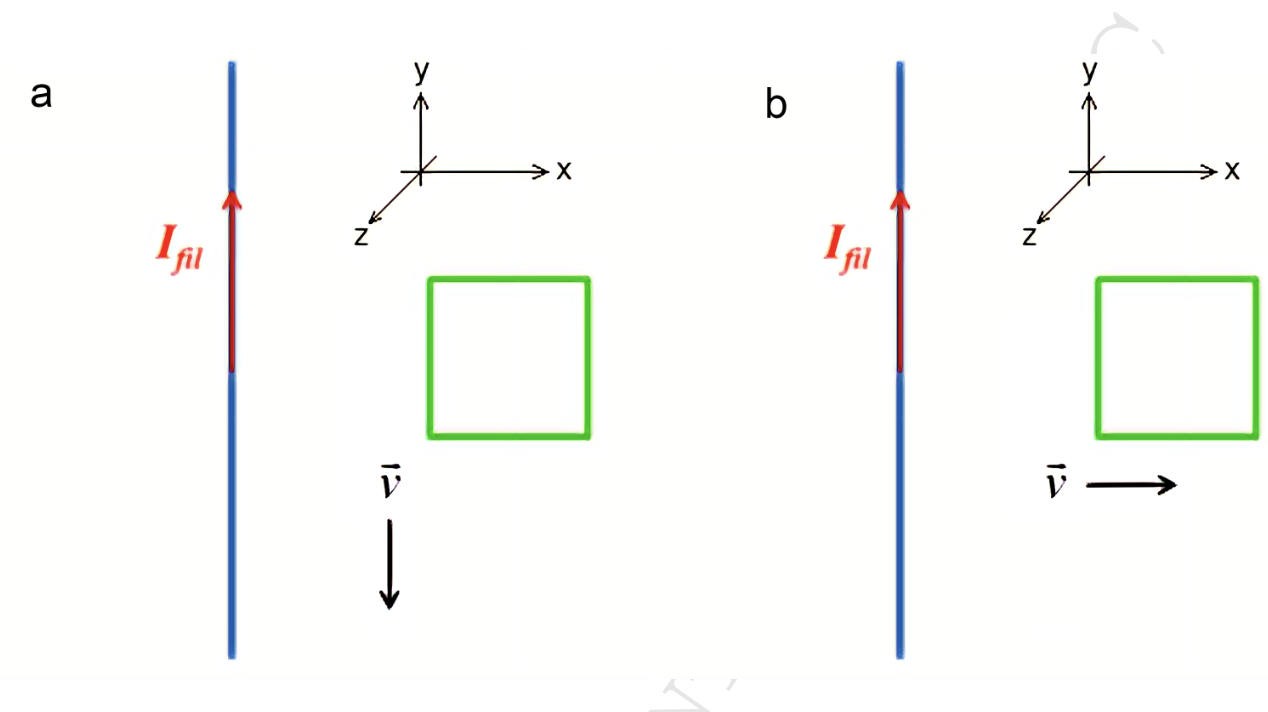
\includegraphics[width=14cm]{imagenes/3.png}
			\caption{Espira e hilo de corriente de la cuestión 3, apartados a) y b)}
		\end{figure} 

		{ \color{blue} 
			\textbf{NOTA:} Todas las fórmulas de esta cuestión han sido tomadas del libro \textit{Magnetostática e inducción electromagnética}.
		}

		\begin{enumerate}[label=\alph*)] 
			\item Razone si se induce corriente en la espira si esta se mueve paralela al hilo y, en caso afirmativo, el sentido de la corriente inducida.

				{ \color{blue} 
					Para determinar si se induce corriente, primero debemos analizar el campo magnético que atraviesa la espira. El campo de inducción magnética creado por un hilo rectilíneo infinito viene dado por la Ecuación 13: $\vec{B}(r) = \frac{\mu_0 I}{2\pi r} \hat{\phi}$. Al aplicar la regla de la mano derecha, a la derecha del hilo, donde se encuentra la espira, este campo es perpendicular al plano $XY$ y entra en la página.

					El flujo magnético $\Phi$ que atraviesa la espira se define mediante la Ecuación 41: $\Phi = \int_S \vec{B} \cdot d\vec{S}$. Si la espira se mueve de forma paralela al hilo a lo largo del eje $Y$, la distancia radial $r$ de cada punto de la espira al hilo se mantiene constante. Dado que la magnitud del campo $\vec{B}$ solo depende de la distancia $r$, el campo magnético y, por consiguiente, el flujo magnético a través de la espira permanecen constantes a lo largo del tiempo.

					La ley de inducción de Faraday-Lenz establece que la fuerza electromotriz inducida depende de la variación temporal del flujo, según indica la Ecuación 53: $\varepsilon_{ind} = - \frac{d\Phi}{dt}$. Dado que el flujo magnético no experimenta variación con el tiempo ($d\Phi/dt = 0$), \textbf{no se induce ninguna fuerza electromotriz y, por tanto, no se induce corriente en la espira} al moverse paralela al hilo.
				}

			\item Si ahora la espira se aleja del hilo en el sentido positivo del eje $X$ en vez de moverse paralela, indique si se induce corriente en la espira como se indica en la Figura 2 y, en caso afirmativo, dibújelo indicando su sentido.

				{ \color{blue}
					Al alejar la espira del hilo en el sentido positivo del eje $X$, la distancia $r$ entre el hilo de corriente y el área de la espira aumenta de forma continua. Como describe la Ecuación 13, $\vec{B}(r) = \frac{\mu_0 I}{2\pi r} \hat{\phi}$, el campo magnético es inversamente proporcional a dicha distancia radial. Por tanto, a medida que la espira se aleja, la magnitud del campo magnético que la atraviesa va disminuyendo progresivamente.

					Dado que la magnitud del campo disminuye, el flujo magnético entrante a través de la superficie de la espira también se reduce. La relación que rige las consecuencias de este fenómeno es la ley de inducción de Faraday-Lenz enunciada en la Ecuación 53: $\varepsilon_{ind} = - \frac{d\Phi}{dt}$. Puesto que ahora existe una variación temporal del flujo, \textbf{sí se induce una corriente eléctrica en la espira}.

					Para deducir el sentido de esta corriente inducida, debemos aplicar el principio subyacente en el signo negativo de la Ecuación 53, conocido como ley de Lenz: \textit{"el signo negativo se conoce como ley de Lenz y hace referencia a que la corriente inducida tendrá el sentido tal que generará un campo magnético que se opondrá a la variación de flujo"}. 

					Como el flujo original que entra en el plano de la espira está disminuyendo, la espira debe oponerse a este cambio creando más flujo entrante. Por lo tanto, generará un campo magnético inducido, $\vec{B}_{ind}$), que también entre en el plano de la pantalla. Si aplicamos la regla de la mano derecha, para que la corriente genere un campo magnético que se adentre en la página en el interior de la espira, \textbf{la corriente inducida debe circular obligatoriamente en sentido horario}.

					\begin{figure}[H]
						\centering
						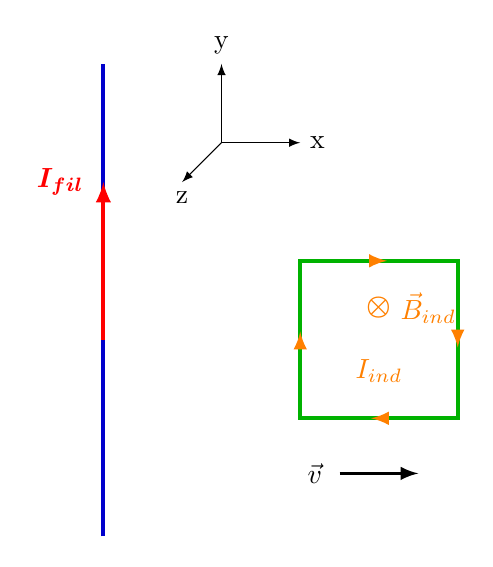
\begin{tikzpicture}[>=latex]
							% Sistema de coordenadas (esquina superior derecha)
							\draw[->] (1.5, 3) -- (2.5, 3) node[right] {x};
							\draw[->] (1.5, 3) -- (1.5, 4) node[above] {y};
							\draw[->] (1.5, 3) -- (1, 2.5) node[below] {z};

							% Hilo conductor (azul)
							\draw[line width=1.5pt, color=blue!80!black] (0, -2) -- (0, 4);

							% Corriente en el hilo (flecha roja)
							\draw[->, line width=1.5pt, color=red] (0, 0.5) -- (0, 2.5) node[left=3pt] {$\boldsymbol{I_{fil}}$};

							% Espira (cuadrado verde)
							\draw[line width=1.5pt, color=green!70!black] (2.5, -0.5) rectangle (4.5, 1.5);

							% Vector velocidad (flecha negra alejándose)
							\draw[->, line width=1.2pt] (3, -1.2) -- (4, -1.2);
							\node[left] at (2.9, -1.2) {$\vec{v}$};

							% ---------------------------------------------------------
							% Respuesta a la inducción
							% ---------------------------------------------------------

							% Flechas naranjas sobre la espira indicando SENTIDO HORARIO
							\draw[->, line width=1.2pt, color=orange] (3.4, 1.5) -- (3.6, 1.5); % Arista superior
							\draw[->, line width=1.2pt, color=orange] (4.5, 0.6) -- (4.5, 0.4); % Arista derecha
							\draw[->, line width=1.2pt, color=orange] (3.6, -0.5) -- (3.4, -0.5); % Arista inferior
							\draw[->, line width=1.2pt, color=orange] (2.5, 0.4) -- (2.5, 0.6); % Arista izquierda

							% Etiqueta de la corriente inducida
							\node[color=orange, font=\bfseries] at (3.5, 0.1) {$I_{ind}$};

							% Símbolo del campo magnético inducido (entrante al papel)
							\node[color=orange] at (3.5, 0.9) {$\boldsymbol{\otimes}$};
							\node[color=orange, right] at (3.65, 0.9) {$\vec{B}_{ind}$};

						\end{tikzpicture}
						\caption{Esquema mostrando el sentido horario de la corriente inducida ($I_{ind}$) al alejarse la espira.}
					\end{figure}
				}
		\end{enumerate}
	\end{problem}

	% --- Exercise 4 ---
	\begin{problem}[Cuestión 4]
		Un transformador elevador diseñado para la etapa de alta tensión de una máquina de tomografía computarizada recibe una tensión de alimentación primaria $V_1$ de 250 V. El objetivo es elevar esta tensión hasta $V_2 = 1000 \text{ V}$ para prepararla para la última etapa de multiplicación que alimentará el tubo de RX.

		Sabemos que el flujo magnético total medido en la bobina secundaria del transformador $\left (\Phi_2 \right)$ es de 2,4 Wb. Si el diseño establece que el flujo que atraviesa cada espira $\Phi$ del transformador es de 0,004 Wb, calcule el número de espiras de las bobinas de la primaria, $N_1$, y de la secundaria, $N_2$, que hacen posible esta transformación de voltaje.

		{ \color{blue} 
			\textbf{NOTA:} Todas las fórmulas de esta cuestión han sido tomadas del libro \textit{Magnetostática e inducción electromagnética}.
		}

		{ \color{blue}
			Para calcular el número de espiras de ambas bobinas, analizamos la bobina secundaria. La expresión que relaciona el flujo magnético total en la bobina secundaria con el flujo que atraviesa cada espira es la Ecuación 83: $\Phi_2 = N_2 \Phi$.

			Al despejar el número de espiras $N_2$ de esta expresión y sustituir los datos proporcionados por el enunciado ($\Phi_2 = 2,4 \text{ Wb}$ y $\Phi = 0,004 \text{ Wb}$), obtenemos las espiras de la secundaria:
			\begin{equation*}
				N_2 = \frac{\Phi_2}{\Phi} = \frac{2,4}{0,004} = \mathbf{600 \text{ espiras}}
			\end{equation*}

			A continuación, para hallar el número de espiras de la bobina primaria, nos basaremos en las propiedades de un transformador ideal. La ley que vincula la caída de tensión y el número de espiras en el primario y el secundario está descrita por la Ecuación 88: $\frac{V_1}{V_2} = \frac{N_1}{N_2}$.

			Aislamos la incógnita $N_1$ en la fórmula y sustituimos los valores numéricos conocidos ($V_1 = 250 \text{ V}$, $V_2 = 1000 \text{ V}$ y $N_2 = 600$) para llegar al resultado final:
			\begin{equation*}
				N_1 = N_2 \cdot \frac{V_1}{V_2} = 600 \cdot \frac{250}{1000} = 600 \cdot 0,25 = \mathbf{150 \text{ espiras}}
			\end{equation*}

			Por lo tanto, la bobina del primario tendrá \textbf{150 espiras} y la del secundario \textbf{600 espiras}.
		}
	\end{problem}

	% -- Exercise 5 ---
	\begin{problem}[Cuestión 5]
		Las fuentes de alimentación de los dispositivos electrónicos están formadas por diodos que contienen una unión p-n de silicio. La región p tiene una concentración $N_A = 1 \times 10^{16} \text{ cm}^{-3}$  y para la región n la concentración es de $N_D = 2 \times 10^{17} \text{ cm}^{-3}$.

		Calcule la anchura de la zona de vaciado de la unión p-n.

		\textbf{Datos:} $k_B T/q= 0,02586 \text{ V}, \, q=1,602 \times 10^{-19} \text{ C}, \, n_i = 1,45 \times 10^{10} \text{ cm}^{-3} \text{ y } \varepsilon_r = 11,8$.

		{ \color{blue} 
			\textbf{NOTA:} Todas las fórmulas de esta cuestión han sido tomadas del libro \textit{Materiales y dispositivos semiconductores}.
		}

		{ \color{blue} 
			Para calcular la anchura de la zona de vaciado, primero debemos hallar el potencial intrínseco de la unión, $V_{bi}$. La fórmula que relaciona este potencial con las concentraciones de impurezas es la Ecuación 39: $V_{bi} = \frac{k_B T}{q} \ln \left( \frac{N_A \cdot N_D}{n_i^2} \right)$.

			Al sustituir los datos proporcionados por el enunciado, obtenemos el potencial intrínseco:
			\begin{align*}
				V_{bi} &= 0,02586 \cdot \ln \left( \frac{1 \times 10^{16} \cdot 2 \times 10^{17}}{(1,45 \times 10^{10})^2} \right) \\
				&= 0,02586 \cdot \ln \left( \frac{2 \times 10^{33}}{2,1025 \times 10^{20}} \right) \\
				&= 0,02586 \cdot \ln (9,512 \times 10^{12}) \approx \textbf{0,7728 V}
			\end{align*}

			A continuación, utilizamos la Ecuación 40 para determinar la anchura total de la zona de vaciado $W$: $W = \left[ \frac{2 \varepsilon_0 \varepsilon_r V_{bi}}{q} \left( \frac{1}{N_A} + \frac{1}{N_D} \right) \right]^{1/2}$.

			Para obtener el resultado correctamente en metros, expresamos las concentraciones de dopaje $N_A$ y $N_D$ en $\text{m}^{-3}$, tal y como se procede en el cálculo de la zona de vaciado:
			\begin{align*}
				N_A &= 1 \times 10^{16} \text{ cm}^{-3} = 1 \times 10^{22} \text{ m}^{-3} \\
				N_D &= 2 \times 10^{17} \text{ cm}^{-3} = 2 \times 10^{23} \text{ m}^{-3}
			\end{align*}

			Empleamos el valor de la permitividad dieléctrica del vacío $\varepsilon_0 = 8,85 \times 10^{-12} \text{ F/m}$ y sustituimos todos los valores en la ecuación:
			\begin{align*}
				W &= \left[ \frac{2 \cdot 8,85 \times 10^{-12} \cdot 11,8 \cdot 0,7728}{1,602 \times 10^{-19}} \left( \frac{1}{10^{22}} + \frac{1}{2 \times 10^{23}} \right) \right]^{1/2} \\
				&= \left[ \frac{161,38 \times 10^{-12}}{1,602 \times 10^{-19}} \left( 10 \times 10^{-23} + 0,5 \times 10^{-23} \right) \right]^{1/2} \\
				&= \left[ 1,0073 \times 10^9 \cdot \left( 10,5 \times 10^{-23} \right) \right]^{1/2} \\
				&= \left[ 10,577 \times 10^{-14} \right]^{1/2} \\
				&\approx 3,252 \times 10^{-7} \text{ m} = \textbf{0,325 } \boldsymbol{\mu}\textbf{m}
			\end{align*}

			Como conclusión, sabemos que \textbf{la anchura de la zona de vaciado de la unión p-n es de aproximadamente 0,325 $\mu$m}.
		}
	\end{problem}

	% -- Exercise 6 ---
	\begin{problem}[Cuestión 6]
		Razone si las siguientes afirmaciones son ciertas o falsas:

		\begin{enumerate}[label=\alph*)] 
			\item Una puerta lógica NAND está compuesta por dos pMOSFETs conectados en paralelo y dos nMOSFETS conectados en serie, fabricados en un mismo sustrato de semiconductor.

				{ \color{blue} 
					\textbf{Verdadera.} Según el libro \textit{Materiales y dispositivos semiconductores}, la tecnología conocida como CMOS (complementary metal-oxide-semiconductor) permite fabricar circuitos lógicos combinando transistores nMOSFET y pMOSFET complementarios "en un mismo sustrato mediante diferentes pasos tecnológicos". En el caso de la puerta lógica NAND, el texto detalla que "se combinan dos nMOSFET con dos pMOSFET para tener dos entradas y una salida" y que en su esquema "los dos pMOSFET están en paralelo y los dos nMOSFET están en serie".
				}

			\item Un fotodetector de silicio (con energía del gap $E_g = 1,12 \text{ eV}$) se puede utilizar para detectar luz de longitud de onda $\lambda = 1200 \text{ nm}$.

				{ \color{blue} 
					\textbf{Falsa.} Para que un fotodetector genere una fotocorriente a partir de la luz incidente, es necesario que la absorción de un fotón tenga una energía mayor o igual que la anchura de la banda prohibida ($E_{\text{fotón}} \ge E_g$) para poder producir un par $e^- - h^+$. Podemos hallar la energía del fotón despejando la Ecuación 58: $\lambda = \frac{h \cdot c}{E_g} \implies E_{\text{fotón}} = \frac{h \cdot c}{\lambda}$. 

					Al sustituir los valores de la constante de Planck ($h = 6,626 \times 10^{-34} \text{ J}\cdot\text{s}$), la velocidad de la luz ($c = 3 \times 10^8 \text{ m/s}$) y la longitud de onda dada ($\lambda = 1200 \times 10^{-9} \text{ m}$), obtenemos la energía en julios:
					\begin{equation*}
						E_{\text{fotón}} = \frac{6,626 \times 10^{-34} \cdot 3 \times 10^8}{1200 \times 10^{-9}} = 1,6565 \times 10^{-19} \text{ J}
					\end{equation*}

					Para pasar esta energía a electronvoltios (eV), dividimos por la carga elemental del electrón ($q = 1,602 \times 10^{-19} \text{ C}$):
					\begin{equation*}
						E_{\text{fotón}} = \frac{1,6565 \times 10^{-19}}{1,602 \times 10^{-19}} \approx \textbf{1,034 eV}
					\end{equation*}

					Como la energía del fotón incidente ($1,034 \text{ eV}$) es inferior a la energía del gap del silicio ($E_g = 1,12 \text{ eV}$), no se crearán pares $e^- - h^+$ y, en consecuencia, este fotodetector de silicio no podrá detectar luz a $1200 \text{ nm}$.
				}

			\item Un semiconductor con una densidad de impurezas donadoras $N_D$ es de tipo p y las densidades de electrones de conducción y huecos son $n = n_i$ y $p = N_D$.

				{ \color{blue} 
					\textbf{Falsa.} Al introducir una densidad de impurezas donadoras ($N_D$) en un semiconductor extrínseco, este pasa a tener más electrones de conducción que huecos, por lo que el semiconductor se denomina de \textbf{tipo n}, no de tipo p. Un semiconductor sólo es de tipo p cuando se le añaden impurezas aceptadoras ($N_A$).

					Además, las densidades de los portadores indicadas no son correctas. En un material de tipo n, casi todos los electrones de conducción provienen de los donadores, haciendo que la densidad de electrones sea $n_n = N_D$, como refleja la Ecuación 10. A su vez, por la ley de acción de masas ($n \cdot p = n_i^2$), la densidad de huecos disminuye y se calcula como $p_n = \frac{n_i^2}{N_D}$, según la Ecuación 14.
				}
		\end{enumerate}
	\end{problem}

	% --- Problem ---
	\begin{problem}[Problema]
		Tenemos una bobina como la de la Figura 3. La bobina tiene $N = 300$ espiras, una longitud de $\ell = 20 \text{ cm}$ y un radio de $r = 10 \text{ mm}$. Se puede considerar que la bobina es infinita ya que su longitud es mucho mayor que su radio. La intensidad de la bobina varía como

		$$i(t) = I_0 \left( 1 + \frac{t}{\tau} \right )$$

		donde $I_0 = 2 \text{ A}$ y $\tau = 20 \text{ s}$.

		(Donde la corriente $i$ se expresa en amperios y el tiempo $t$ en segundos). Calcule:

		\begin{figure}[H]
			\centering
			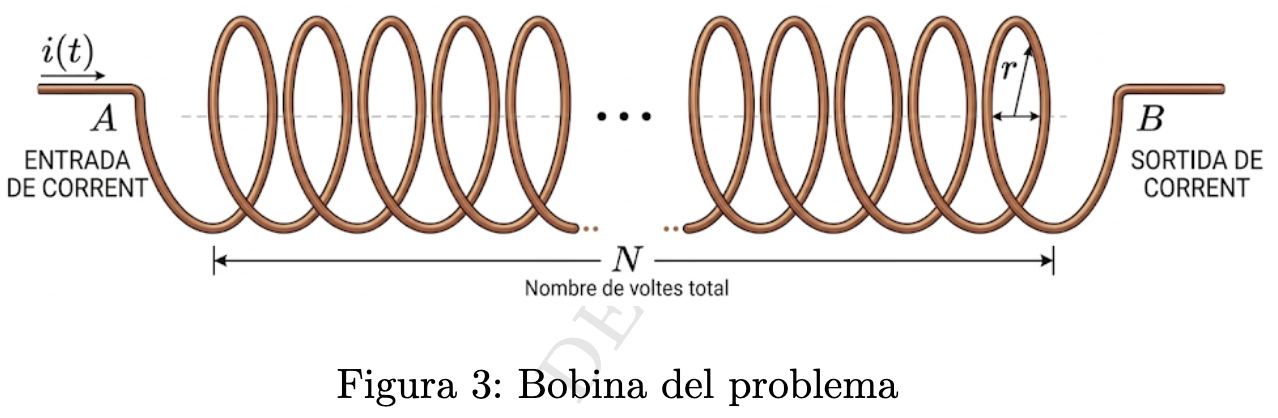
\includegraphics[width=14cm]{imagenes/problema.png}
			\caption{Bobina del problema}
		\end{figure} 

		{ \color{blue} 
			\textbf{NOTA:} Todas las fórmulas de esta cuestión han sido tomadas del libro \textit{Magnetostática e inducción electromagnética}.
		}

		\begin{enumerate}[label=\alph*)] 
			\item La autoinductancia $L$ de la bobina.

				{ \color{blue} 
					Para calcular la autoinductancia $L$ de una bobina que se puede considerar infinita, utilizamos la Ecuación 67: $L = \mu_0 \cdot n^2 \cdot A \cdot \ell$.

					En esta expresión, $\mu_0$ es la permeabilidad magnética del vacío, cuyo valor es $4\pi \times 10^{-7} \text{ H/m}$; $n$ es la densidad de espiras; $A$ es el área transversal de la bobina; y $\ell$ es su longitud.

					Primero calculamos el área transversal $A$ a partir del radio de la bobina ($r = 10 \text{ mm} = 0,01 \text{ m}$):
					\begin{equation*}
						A = \pi \cdot r^2 = \pi \cdot (0,01)^2 = \pi \cdot 10^{-4} \text{ m}^2
					\end{equation*}

					Tras ello, calculamos la densidad de espiras $n$, que equivale al número total de espiras $N$ dividido por la longitud $\ell = 20 \text{ cm} = 0,2 \text{ m}$:
					\begin{equation*}
						n = \frac{N}{\ell} = \frac{300}{0,2} = 1500 \text{ espiras/m}
					\end{equation*}

					Por último, sustituimos todos los valores en la Ecuación 67 para obtener la autoinductancia:
					\begin{align*}
						L &= (4\pi \times 10^{-7}) \cdot (1500)^2 \cdot (\pi \times 10^{-4}) \cdot 0,2 \\
						&= (4\pi \times 10^{-7}) \cdot (2,25 \times 10^6) \cdot (\pi \times 10^{-4}) \cdot 0,2 \\
						&= 1,8 \pi^2 \times 10^{-5} \text{ H} \approx \textbf{1,777} \times \textbf{10}^{-4} \textbf{ H}
					\end{align*}
				}

			\item La fuerza electromotriz inducida en la bobina.

				{ \color{blue} 
					Para determinar la fuerza electromotriz inducida ($\varepsilon$), nos basamos en la ley de Faraday-Lenz. Tal como se expresa en la Ecuación 68, cuando circula una corriente variable en el tiempo por una bobina, la fuerza electromotriz inducida depende de su autoinductancia y de la variación temporal de la intensidad: $\varepsilon = -L \frac{dI}{dt}$.

					Dado que la intensidad varía según la expresión $i(t) = I_0 \left( 1 + \frac{t}{\tau} \right)$, donde $\tau = 20 \text{ s}$ es la constante de tiempo dada por el enunciado, calculamos primero su derivada respecto al tiempo:
					\begin{equation*}
						\frac{dI}{dt} = \frac{d}{dt} \left[ 2 \left( 1 + \frac{t}{20} \right) \right] = \frac{2}{20} = 0,1 \text{ A/s}
					\end{equation*}

					Sustituimos el valor de la autoinductancia $L$ obtenido en el apartado anterior y la derivada de la corriente en la Ecuación 68:
					\begin{equation*}
						\boxed{\varepsilon = - (1,8 \pi^2 \times 10^{-5}) \cdot 0,1 = -1,8 \pi^2 \times 10^{-6} \text{ V} \approx \textbf{-1,777} \times \textbf{10}^{-5} \textbf{ V}}
					\end{equation*}

					El signo negativo indica que la corriente inducida y su fuerza electromotriz asociada tendrá un sentido tal que generará un campo magnético que se opondrá a la variación de flujo, según la ley de Lenz.
				}

			\item La energía almacenada en la bobina para $t = 10 \text{ s}$.

				{ \color{blue} 
					La energía magnética almacenada en una bobina se puede calcular mediante la Ecuación 71: $U_m = \frac{1}{2} L I^2$.

					Primero, evaluamos la intensidad de la corriente en el instante $t = 10 \text{ s}$:
					\begin{equation*}
						i(10) = 2 \left( 1 + \frac{10}{20} \right) = 2 \cdot 1,5 = 3 \text{ A}
					\end{equation*}

					Sustituimos el valor de $L$ y el de la corriente en la Ecuación 71:
					\begin{align*}
						U_m(10) &= \frac{1}{2} \cdot (1,8 \pi^2 \times 10^{-5}) \cdot (3)^2 \\
						&= 0,9 \pi^2 \times 10^{-5} \cdot 9 \\
						&= 8,1 \pi^2 \times 10^{-5} \text{ J} \approx \textbf{7,994} \times \textbf{10}^{-4} \textbf{ J}
					\end{align*}
				}

			\item Represente gráficamente la evolución de la energía magnética almacenada, $U_m (t)$, en el intervalo de tiempo comprendido entre $t = 0$ y $t = 20 \text{ s}$. Indique claramente el valor de la energía en los instantes $t = 0$, $t = 10 \text{ s}$ y $t = 20 \text{ s}$. Relacione la forma de la gráfica con la energía proporcionada al sistema y explique el efecto de duplicar la corriente.

				{ \color{blue} 
					Para representar gráficamente y analizar la evolución de la energía magnética almacenada $U_m(t)$, primero calculamos el valor de la energía en los instantes solicitados ($t = 0 \text{ s}$, $t = 10 \text{ s}$ y $t = 20 \text{ s}$) aplicando la Ecuación 71: $U_m = \frac{1}{2} L I^2$.

					\begin{itemize}
						\item \textbf{En $\mathbf{t = 0 \text{ s}}$:} \\ 
						$i(0) = 2 \left( 1 + \frac{0}{20} \right) = 2 \text{ A} \implies U_m(0) = \frac{1}{2} L (2)^2 = 2L = 3,6 \pi^2 \times 10^{-5} \text{ J} \approx \textbf{3,553} \times \textbf{10}^{-4} \textbf{ J}$

						\item \textbf{En $\mathbf{t = 10 \text{ s}}$:} \\
						$U_m(10) \approx \textbf{7,994} \times \textbf{10}^{-4} \textbf{ J}$ (calculado en el apartado anterior).

						\item \textbf{En $\mathbf{t = 20 \text{ s}}$:} \\
						$i(20) = 2 \left( 1 + \frac{20}{20} \right) = 4 \text{ A} \implies U_m(20) = \frac{1}{2} L (4)^2 = 8L = 14,4 \pi^2 \times 10^{-5} \text{ J} \approx \textbf{1,421} \times \textbf{10}^{-3} \textbf{ J}$
					\end{itemize}

					A continuación se presenta la representación gráfica de $U_m(t)$:

					\begin{center}
						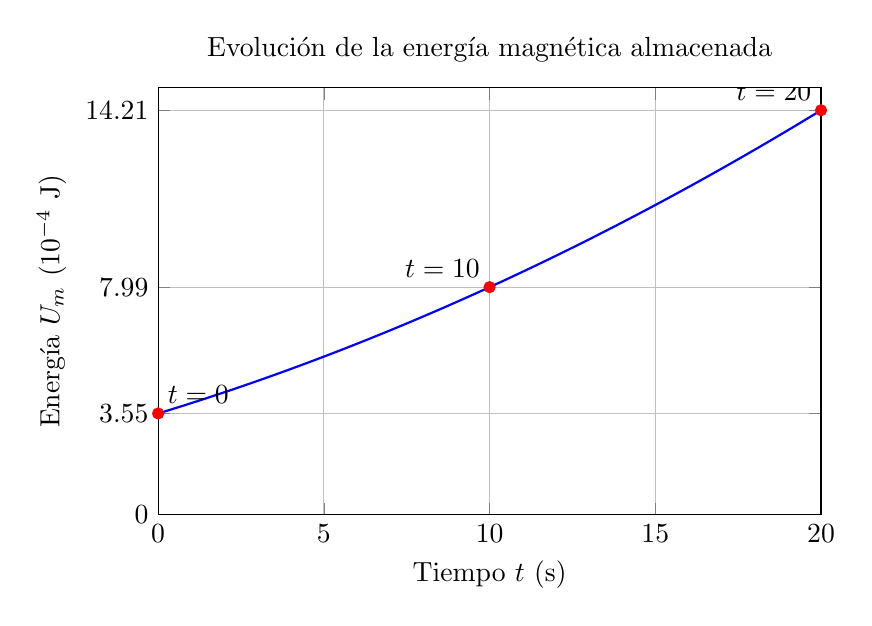
\begin{tikzpicture}
							\begin{axis}[
								title={Evolución de la energía magnética almacenada},
								xlabel={Tiempo $t$ (s)},
								ylabel={Energía $U_m$ ($10^{-4}$ J)},
								xmin=0, xmax=20,
								ymin=0, ymax=15,
								grid=major,
								xtick={0, 5, 10, 15, 20},
								ytick={0, 3.55, 7.99, 14.21},
								legend pos=north west,
								width=10cm,
								height=7cm
							]
							\addplot[
								domain=0:20, 
								samples=100, 
								color=blue,
								thick
							]
							{0.5 * 1.7765 * (2*(1 + x/20))^2};

							\addplot[
								only marks,
								mark=*,
								color=red
							]
							coordinates {
								(0, 3.553)
								(10, 7.994)
								(20, 14.212)
							};
							\node[above right] at (axis cs:0, 3.553) {$t=0$};
							\node[above left] at (axis cs:10, 7.994) {$t=10$};
							\node[above left] at (axis cs:20, 14.212) {$t=20$};
							\end{axis}
						\end{tikzpicture}
					\end{center}

					Como se deduce de la Ecuación 71, la energía magnética es directamente proporcional al cuadrado de la intensidad de corriente ($U_m \propto I^2$). Como la intensidad $i(t)$ aumenta de forma lineal con el tiempo, al elevarla al cuadrado obtenemos una función cuadrática respecto a la variable temporal. Por este motivo, la gráfica que ilustra la acumulación de energía proporcionada al sistema presenta la forma de una \textbf{parábola creciente}.

					Respecto al efecto de duplicar la corriente, dado que la energía está relacionada con el cuadrado de dicha intensidad, \textbf{si la corriente se multiplica por dos, la energía magnética almacenada en el sistema se multiplica por cuatro} ($2^2 = 4$). Este comportamiento se observa de forma evidente al comparar los instantes $t=0$ y $t=20$ s. Durante este intervalo de tiempo, la corriente pasa de $2 \text{ A}$ a $4 \text{ A}$, lo que desencadena que la energía asociada aumente de su valor inicial de $2L$ al valor de $8L$, cuadruplicando exactamente el almacenamiento energético en la bobina.
				}
		\end{enumerate}
	\end{problem}
\end{document}